% VARIABLES %%%
% \date{\today}
\def\longTitle{Théorème de Pythagore - Sens direct}
\def\shortTitle{\MakeUppercase{\longTitle}}

\setcounter{seq}{2}
\bseq{\longTitle}

\setgrade{4e}
\def\imgPath{enseignement/4e/theoreme-de-pythagore/sens-direct/}
%%

\def\ym{\href{https://www.maths-et-tiques.fr/telech/19Pyth1.pdf}{Yvan Monka}}

\avspace{0.1cm}

\obj{
    \item Utiliser la calculatrice pour déterminer une valeur approchée de la racine carrée d'un nombre positif.
    \item Utiliser la racine carrée d'un nombre positif en lien avec des situations géométriques.
    \item Utiliser le sens direct du Théorème de Pythagore.
}

\scn{Decouvrir l'égalité de Pythagore}
\bsec{Egalité de Pythagore}

\slide{qf}{
    \dividePage{
        \begin{enumerate}
            \item Peut-on construire un triangle $ABC$ avec:
            \begin{enumerate}
                \item $AB = 5cm \pv BC = 11cm \pv AC = 4cm$
                \item $AB = 8cm \pv BC = 9cm \pv AC = 6cm$
            \end{enumerate}
        \end{enumerate}
    }{
        \imgp{mi-c4/qf-5p426}[7cm]
    }
}

\slide{exo}{
    \bvspace{-0.5cm}
    \act{}{
        \bvspace{-0.5cm}
        \dividePage{%
            \imgp{activite-decouverte-fig}[5cm]
        }
        {
            \ifBeamer{\small}
            \begin{enumerate}
                \item Donner une expression mathématique permettant de calculer l'aire des carrés 1; 2 et 3.
                \item Découper les quatre triangles et le carré fournis en annexe.
                \item Disposer les quatre triangles dans le carré afin de former deux nouveaux carrés.
                \item Quelles sont les aires des deux carrés formés ?
            \end{enumerate}
        }[0.35]
    }[\href{https://drive.google.com/drive/folders/1ipPqxysYc8GHNOIT0u6HSi8cAnUiYfxx}{Audrey Belay}]
}

\slide{exo}{
    \begin{enumerate}\setcounter{enumi}{4}
        \item Disposer les quatre triangles dans le carré afin de former un seul carré.
        \item Quelle est l'aire de ce carré ?
        \item Quelle relation peut-on établir entre les aires des carrés 1, 2 et l'aire du carré 3 ?
        \item Quelle relation peut-on établir entre les longueurs $a$, $b$ et $c$ ?
    \end{enumerate}
    \ifArticle{Annexe:\imgp{activite-decouverte-print}[6cm]}
}

\slide{cr}{
    \sseq\ssec
    \df{}{
        Dans un triangle rectangle, le côté opposé à l'angle droit est appelé \key{hypoténuse}.
    }[\href{https://fr.wikipedia.org/wiki/Hypoténuse}{Wikipédia}]
}

\slide{cr}{
    \setboolean{showID}{false}
    \thm{de Pythagore}{
        \Si un triangle est rectangle,
        \Alors le carré de la longueur de l'hypoténuse est égal à la somme des carrés des longueurs des deux autres côtés.
        \color{black}
        \begin{center}
            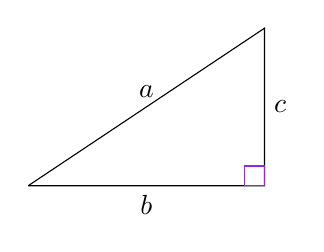
\begin{tikzpicture}[scale=1]%,cap=round,>=latex]
                \coordinate (A) at (-1.5cm,-1.cm);
                \coordinate (C) at (1.5cm,-1.0cm);
                \coordinate (B) at (1.5cm,1.0cm);
                \draw (A) -- node[above] {$a$} (B) -- node[right] {$c$} (C) -- node[below] {$b$} (A);
                \draw[color = BlueViolet] (1.25cm,-1.0cm) rectangle (1.5cm,-0.75cm);
            \end{tikzpicture}\\
            \color{ForestGreen}$c^2=a^2+b^2$
        \end{center}
    }
    \setboolean{showID}{true}
}

\slide{cr}{
    \expl{}{
        Soit $ABC$ un triangle rectangle en $A$, tel que $AB = 6$, $AC = 8$, $BC=10$.
        Verifier si le triangle $ABC$ respecte bien l'égalité de Pythagore.
    }
}

\def\imgPrefix{mi-c4/exo-}
\exoSlide{3p430,4p430}[7cm][2][\mi]

\scn{Decouvrir la racine carré}

\def\imgPrefix{mi-c4/qf-}
\exoSlide{3p426}[10cm][1][\mi][qf]

\bsec{Racine carré}

\slide{exo}{
    \act{}{
        \begin{enumerate}
            \item Calculer l'aire d'un carré de côté:
            \multiColEnumerate{4}{
                \item $3\cm$ \item $12\cm$ \item $5,5\cm$ \item $x\cm$
            }
            \item Trouvé le côté d'un carré d'aire:
            \multiColEnumerate{4}{
                \item $4\cmd$ \item $25\cmd$ \item $1\cmd$ \item $169\cmd$
            }
            \item Encadrer par deux entiers le côté d'un carré d'aire $40\cmd$.
            \item Trouver le côté d'un carré d'aire $20.25\cmd$.
            \item Approcher au centième près le côté d'un carré d'aire $2\cmd$.
        \end{enumerate}
    }
}

\slide{cr}{
    \ssec
    \df{}{
        La \key{racine carrée} d'un nombre positif $x$ est l'unique nombre positif qui,
        lorsqu'il est multiplié par lui-même,
        donne $x$.
    }[\wiki{Racine_carrée}]

    \df{}{
        Un \key{carré parfait} est le carré d'un entier naturel.
    }[\wiki{Carré_parfait}]
}

\scn{Calculer une longueur grace au Théorème de Pythagore}

\def\imgPrefix{mi-c4/qf-}
\exoSlide{1p430}[8cm][1][\mi][qf]

\expl{}{
    Soit $ABC$ un triangle rectangle en $A$, tel que $AB = 3$ et $AC = 4$.
    Déterminer $BC$.
}

\slide{exo}{
    \exo{}{%
        Un professeur d'EPS trace un circuit de course à pied avec des plots :
        \begin{itemize}
            \item le plot n°2 est situé à 36 m au nord du plot n°1, qui est le plot de départ ;
            \item le plot n°3 est situé à 69 m à l'est du plot n°2 ;
            \item le plot n°4 est situé à 72 m au sud du plot n°3.
        \end{itemize}
        Chaque élève va d'un plot au suivant en ligne droite,
        et parcourt un certain nombre de fois le circuit 1-2-3-4-1.
        Il continue sur le même circuit jusqu'au plot d'arrivée,
        placé sur ce circuit de telle sorte le trajet total ait une longueur de 1,5 km.
        \\Où le professeur doit-il placer le plot d'arrivée ?
        \\Combien de fois un élève doit-il parcourir le circuit ?
    }[\href{https://eduscol.education.fr/document/17305/download\#page=8}
    {Utiliser les notions de géométrie plane pour démontrer}]
}

\slide{exo}{
    \exo{}{

    }[\href{https://blogdemaths.wordpress.com/2015/06/27/jusquou-peut-on-voir-a-lhorizon/}{Jusqu'où peut on voir à l'horizon?}]
}